\documentclass[french,10pt]{beamer}
\usetheme{Darmstadt}
\usepackage[utf8]{inputenc}
\usepackage[T1]{fontenc}
\usepackage{lmodern}
\usepackage{babel}
\usepackage{xcolor}   
\usepackage{amsmath}
\usepackage{booktabs}
\usepackage{amsfonts}
\usepackage{amssymb}
\usepackage{graphicx}
\usepackage{listings}
\usepackage{color}
\date{}
\usepackage{float}
\restylefloat{table}
\usepackage{textcomp}
\usepackage{pgfplots,pgfplotstable}
\usepackage{url}
\usepackage{tikz}
\usetikzlibrary{arrows,backgrounds,mindmap,positioning,shadows,shapes}
\definecolor{listinggray}{gray}{0.9}
\definecolor{lbcolor}{rgb}{0.9,0.9,0.9}

\pgfplotstableset{
every head row/.style={before row=\toprule,after row=\midrule},
every last row/.style={after row=\bottomrule}}


\lstset{
	backgroundcolor=\color{lbcolor},
	tabsize=4,
	rulecolor=,
	language=C++,
        basicstyle=\scriptsize,
        upquote=true,
        aboveskip={0.5\baselineskip},
        columns=fixed,
        showstringspaces=false,
        extendedchars=true,
        breaklines=true,
        prebreak = \raisebox{0ex}[0ex][0ex]{\ensuremath{\hookleftarrow}},
        frame=single,
        showtabs=false,
        showspaces=false,
        showstringspaces=false,
        identifierstyle=\ttfamily,
        keywordstyle=\color[rgb]{0,0,1},
        commentstyle=\it\tt\color[rgb]{0.133,0.545,0.133},
        stringstyle=\color[rgb]{0.627,0.126,0.941},
        inputencoding=utf8
        }

\lstset{escapeinside={(*@}{@*)}}
\lstset{includerangemarker=false,rangeprefix=\/\/\#\ ,% curly left brace plus space
  rangesuffix=\ \#}% space plus curly right brace

\title{Présentation de stage}
\subtitle{Wrapping Python}
\author{LANTZ Thomas\\
		M1 CSMI}
\institute{UFR de Mathématiques et d'Informatique de Strasbourg}
\date{\today}



\begin{document}

\frame{\titlepage}

\begin{frame}
\tableofcontents
\end{frame}

\section{Présentation du sujet}
\begin{frame}
\frametitle{Présentation du sujet}
\begin{itemize}
\item But : Wrapper le code provenant de Feel++ pour pouvoir l'utiliser en Python.
\vspace{1 cm}
\item Utilité : Réduire le temps de compilation nécessaire à chaque modification du code.
(Python interprété / C++ compilé)
\end{itemize}
\end{frame}

\section{Principe du Wrapping Python}
\begin{frame}[fragile]
\frametitle{Principe du Wrapping Python}
\begin{itemize}
\item Récupérer du code déjà implémenté pour construire et générer une librairie utilisable dans un autre langage.
\begin{tabular}{p{5cm}p{6cm}}
    			\begin{small}\begin{lstlisting}
	char const* greet()
{
   return "hello, world";
}
\end{lstlisting}\end{small}
			&    
\begin{small}		
\begin{lstlisting}
		>>> import hello_ext
>>> print hello_ext.greet()
hello, world
\end{lstlisting}
\end{small}
    \end{tabular}
\item Utilisation de librairies déjà existantes permettant le passage et la compatibilité entre ces 2 langages (Boost.Python, SWIG, ....)

\end{itemize}
\end{frame}

\section{La librairie Boost.Python}
\begin{frame}[fragile]
\frametitle{La librairie Boost.Python}
\begin{itemize}
\item Librairie C++ permettant de transposer du code entre les langages C++ et Python.
\vspace{1 cm}
\item Utilisation : 
\end{itemize}
\begin{lstlisting}
#include <boost/python.hpp>
#include <mpi4py/mpi4py.h>

BOOST_PYTHON_MODULE("libName")
{
 if (import_mpi4py()<0) return ;
 .....
 .....
}
\end{lstlisting}
\end{frame}

\section{Wrapping des classes}
\begin{frame}[fragile]
\frametitle{Wrapping des classes}
\begin{itemize}
\item Syntaxe : \\
\begin{lstlisting}
class_<"info_sur_la_classe">("Name",init<arg>());
\end{lstlisting}
\item Pourquoi : 
\begin{itemize}
\item Initialisation du type en Python.
\item Permet le création d'objets de ce type.
\item Permet l'utilisation des méthodes propres à la classe.
\end{itemize}
2 cas présents ici :
\item Classes simples :
\begin{lstlisting}
class_<Feel::detail::Environment,boost::noncopyable>("Environment",no_init);
\end{lstlisting}
\item Classes avec template :
\begin{lstlisting}
class_<Feel::Mesh<Feel::Simplex<2>>,boost::noncopyable>("Mesh",init<>())
\end{lstlisting}
\end{itemize}
\end{frame}

\section{Wrapping des méthodes}
\begin{frame}[fragile]
\frametitle{Wrapping des méthodes}
3 cas possibles :
\begin{itemize}
\item méthodes libres :
\begin{lstlisting}
def("exe1",exe);
\end{lstlisting}
\item méthodes d'instances :
\begin{lstlisting}
class_<A>("A",no_init)
.def("exe1",A::exe);
\end{lstlisting}
\item méthodes de classes :
\begin{lstlisting}
class_<A>("A",no_init)
.def("exe1",A::exe)
.staticmethod("exe1");
\end{lstlisting}
\end{itemize}
\end{frame}

\subsection{Méthodes avec des arguments par défaut}
\begin{frame}[fragile]
\frametitle{Méthodes avec arguments par défaut}
\begin{itemize}
\item Méthodes avec des arguments par défaut
\begin{itemize}
\item Soucis : Perte des valeurs données par défaut
\item Résolution : Création de sous-méthodes appelant cette méthode avec les différentes combinaisons d'arguments voulues.
\item Ex : Méthode boundaryelments (Mesh,uint16\_type,uint16\_type )
\begin{lstlisting}
template<typename MeshType>
boost::tuple<mpl::size_t<MESH_ELEMENTS>,
typename MeshTraits<MeshType>::location_element_const_iterator,
typename MeshTraits<MeshType>::location_element_const_iterator>
boundaryelements_w( MeshType const& mesh)
{
return boundaryelements(mesh);
}
\end{lstlisting}
\end{itemize}
\end{itemize}
\end{frame}

\subsection{Méthodes avec templates}
\begin{frame}[fragile]
\frametitle{Méthodes avec templates}
\begin{itemize}
\item Méthodes avec templates
\begin{itemize}
\item Soucis : Pas d'équivalent aux templates en Python
\item Résolution : Création de sous-méthodes appelant cette méthode avec tout les templates complétés par les  valeurs voulues.
\item Ex : méthode unitSquare ( renvoie un boost$::$shared\_ptr<MeshType>)
\begin{lstlisting}
boost::shared_ptr<Mesh<Simplex<2>>> unitSquare_w ()
{
return unitSquare();
}
\end{lstlisting}
\end{itemize}
\end{itemize}
\end{frame}

\subsection{BOOST\_PARAMETER\_FUNCTION}
\begin{frame}[fragile]
\frametitle{BOOST\_PARAMETER\_FUNCTION}
\begin{itemize}
\item BOOST\_PARAMETER\_FUNCTION
\begin{itemize}
\item Soucis : Technique de wrapping différente.
\item Résolution : Création d'une sous-méthode appelant la BOOST\_PARAMETER\_FUNCTION avec les arguments que l'on veut utiliser.
\item Ex : Méthode loadMesh (Mesh,...)
\begin{lstlisting}
boost::shared_ptr<Mesh<Simplex<2>>> loadMesh_w (Mesh<Simplex<2>>* mesh)
{
 return loadMesh(_mesh=mesh);
}
\end{lstlisting}
\end{itemize}
\end{itemize}
\end{frame}

\section{Exemple à traiter}
\begin{frame}[fragile]
\frametitle{Présentation de l'exemple}
Exemple que nous allons traiter ici : mymesh.cpp
\begin{lstlisting}
int main( int argc, char** argv )
{
// initialize Feel++ Environment
Environment env( _argc=argc, _argv=argv,
_about=about( _name="mymesh" ,
_author="Feel++ Consortium",
_email="feelpp-devel@feelpp.org" ) );
//! [load]
// create a mesh with GMSH using Feel++ geometry tool
auto mesh = loadMesh(_mesh=new Mesh<Simplex<2>>);
//! [load]

//! [export]
// export results for post processing
auto e = exporter( _mesh=mesh );
e->addRegions();
e->save();
//! [export]
#endif
} 
\end{lstlisting}
\end{frame}

\subsection{Environment}
\begin{frame}[fragile]
\frametitle{La classe Environment}
\begin{itemize}
\item Constructeur :
\begin{lstlisting}
Environment(ArgumentPack const& args)
\end{lstlisting}
\item Nouveau constructeur :
\begin{lstlisting}
Environment(boost::python::list arg);
\end{lstlisting}
\item Wrapping de la classe et du constructeur:
\begin{lstlisting}
 class_<Feel::detail::Environment,boost::noncopyable>
 ("Environment", init<boost::python::list>())
 .def("worldComm",&Feel::detail::Environment::worldComm,return_value_policy<copy_non_const_reference>())
 .staticmethod("worldComm");
\end{lstlisting}
\end{itemize}
\end{frame}

\subsection{loadMesh}
\begin{frame}[fragile]
\frametitle{La méthode loadMesh}
\begin{itemize}
\item Définition de la méthode :
\begin{lstlisting}
BOOST_PARAMETER_FUNCTION(
( typename Feel::detail::mesh<Args>::ptrtype ),
loadMesh,
tag,
( required
( mesh, *)
)
( optional
( filename, *( boost::is_convertible<mpl::_,std::string> ),
 option(_name="gmsh.filename").template as<std::string>() )
( desc, *,boost::shared_ptr<gmsh_type>() )
 ....
)
\end{lstlisting}
\item Définition d'une sous-méthode :
\begin{lstlisting}
boost::shared_ptr<Mesh<Simplex<2>>> loadMesh_w (Mesh<Simplex<2>>* mesh)
{
return loadMesh(_mesh=mesh);
}
\end{lstlisting}
\item Wrapping de la sous-méthode :
\begin{lstlisting}
def("loadMesh",loadMesh_w);
\end{lstlisting}
\end{itemize}
\end{frame}

\subsection{Mesh}
\begin{frame}[fragile]
\frametitle{La classe Mesh}
\begin{itemize}
\item Définition de la classe :
\begin{lstlisting}
template <typename GeoShape, typename T = double, int Tag = 0>
class Mesh
\end{lstlisting}
\item Wrapping :
\begin{lstlisting}
 class_<Feel::Mesh<Feel::Simplex<2>>,
 boost::shared_ptr<Feel::Mesh<Feel::Simplex<2>>>,
 boost::noncopyable>("Mesh",init<>())
\end{lstlisting}
\end{itemize}
\end{frame}

\subsection{Exporter}
\begin{frame}[fragile]
\frametitle{La méthode exporter}
\begin{itemize}
\item Définition de la classe associée :
\begin{lstlisting}
template<typename MeshType, int N = 1>
class Exporter
\end{lstlisting}
\item Création de la sous-méthode :
\begin{lstlisting}
template<typename MeshType,int N>
void expo_w ( boost::shared_ptr<MeshType> m)
{
auto x=Exporter<MeshType,N>::New();
x->setMesh(m);
x->addRegions();
x->save();
}
\end{lstlisting}
\item Wrapping :
\begin{lstlisting}
def("export",expo_w<Mesh<Simplex<2>>,1>);
\end{lstlisting}
\end{itemize}
\end{frame}

\subsection{Passage en Python}
\begin{frame}[fragile]
\frametitle{Passage en Python}
\begin{itemize}
\item Script Python :
\begin{lstlisting}
#!/usr/bin/python

from mpi4py import MPI
import libPyMesh
import sys

z=libPyMesh.Environment(sys.argv)
s=libPyMesh.Simplex()
m=libPyMesh.Mesh.new()
l=libPyMesh.loadMesh(m)
w=libPyMesh.Environment.worldComm()

x=libPyMesh.export(l);
\end{lstlisting}
\item Résultat :

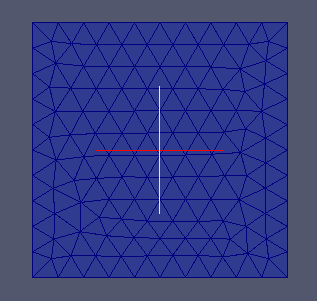
\includegraphics[scale=0.30]{Mesh1.png} 
\end{itemize}
\end{frame}

\section{Wrapping généralisé}

\begin{frame}[fragile]
\frametitle{Création de la librairie Feelpp}
\begin{itemize}
\item But : Créer un module contenant les classes et méthodes, afin de pouvoir utiliser de manière générale l'ensemble du code Feel++ en Python.
\item Création de méthodes contenant la définition du wrapping.
\begin{lstlisting}
template <int n,int N>
void def_wrapper (std::string s)
{
std::ostringstream f;
std::ostringstream g;
if(s.compare("Simplex")==0)
{
f<<"Simplex"<<n;
g<<"MeshS"<<n;
class_<Feel::Simplex<n>>(f.str().c_str(),init<>());
class_<Feel::Mesh<Simplex<n>>,boost::shared_ptr<Feel::Mesh<Simplex<n>>>,boost::noncopyable>(g.str().c_str(),init<>())
.def("new",&Feel::Mesh<Simplex<n>>::New)
.staticmethod("new");
def("loadMesh",loadMesh_w<Mesh<Simplex<n>>>);
def("export",expo_w<Mesh<Simplex<n>>,N>);
}
else ....
}
\end{lstlisting}
\end{itemize}
\end{frame}

\begin{frame}[fragile]
\frametitle{Création de la librairie Feelpp}
\begin{itemize}
\item Utilisation de Boost.Preprocessor et de macros pour générer le module Python.
\begin{itemize}
\item Librairie contenant des macros, utilisées pour générer du code avant le compilation.
\item Utilisation de BOOST\_PP\_REPEAT, définit ainsi
\begin{lstlisting}
 BOOST_PP_REPEAT(n,X,Y)
\end{lstlisting}
appelant la macro X  avec la méthode Y pour des valeurs variant de 0 à $n-1$. 
\end{itemize}
\begin{lstlisting}
#define SIMPLEX(_,n,type) type<n+1,1>("Simplex");
....
BOOST_PYTHON_MODULE(libPyFeelpp)
{
 ...
 BOOST_PP_REPEAT(3,SIMPLEX,def_wrapper)
 ...
}
\end{lstlisting} 
\end{itemize}
\end{frame}

\begin{frame}[fragile]
\frametitle{Utilisation du module Python}
\begin{itemize}
\item Script Python :
\begin{lstlisting}
#!/usr/bin/python

from mpi4py import MPI
import libPyFeelpp
import sys

z=libPyFeelpp.Environment(sys.argv)

m=libPyFeelpp.MeshS3()
l=libPyFeelpp.loadMesh(m)
w=libPyFeelpp.Environment.worldComm()

x=libPyFeelpp.export(l);
\end{lstlisting}
\item Essai du module : Mesh Simplex 3D avec 4 processus
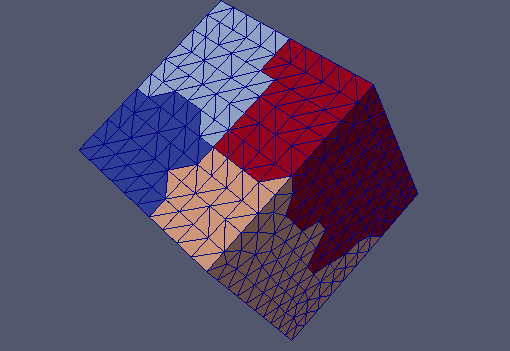
\includegraphics[scale=0.30]{MPI.png} 
\end{itemize}
\end{frame}

\section{Conclusion et Perspective}
\begin{frame}
\frametitle{Conclusion et Perspective}
\begin{itemize}
\item Conclusion
\begin{itemize}
\item  Différentes manières de wrapper les objets que l'on peut rencontrer.
\item Création d'un module général pour Feelpp.
\end{itemize}
\item Perspective d'avenir
\begin{itemize}
\item Améliorer et corriger le module général Feelpp afin de pouvoir utiliser toutes les facettes de la librairie Feel++. 
\end{itemize} 
\end{itemize}
\vspace{1 cm}
Merci de votre attention.
\end{frame}

\end{document}

\begin{frame}[fragile]
\frametitle{Boost.Preprocessor}
\begin{itemize}
\item Librairie contenant des macros, utilisées pour générer du code avant le compilation.
\item Utilisation de BOOST\_PP\_REPEAT, définit ainsi
\begin{lstlisting}
 BOOST_PP_REPEAT(n,X,Y)
\end{lstlisting}
appelant la macro X  avec la méthode Y pour des valeurs variant de 0 à $n-1$. 
\end{itemize}
\end{frame}